% =====================================================================
\section{Implementation}\label{sec:impl}
% =====================================================================

The compiler is a Rust workspace with five crates: \texttt{frontend} (parser, macro expander, desugaring with hygiene resolution, elaborator), \texttt{kernel}, \texttt{mir} (lowering, analyses, optimisations and both code generators), \texttt{cli} (driver, compiler, read--eval--print loop) and \texttt{codegen} (a placeholder; code generation lives in \texttt{mir}).
Table~\ref{tab:scale} gives their sizes and Figure~\ref{fig:pipeline} the pipeline.

\begin{table}[t]
\centering\footnotesize
\caption{Size of the implementation at the pinned commit, in lines of Rust (including comments and blank lines). ``Tests'' are the crates' integration-test directories; unit tests inside \texttt{src/} are counted under ``Source''. The kernel has \NumKernelNonTestLines{} lines of source without its in-crate tests.}
\label{tab:scale}
\begin{tabular}{lrr}\hline
\textbf{Crate} & \textbf{Source} & \textbf{Tests}\\\hline\hline
\texttt{kernel} & \NumKernelSrcLines & \NumKernelTestLines\\
\texttt{frontend} & \NumFrontendSrcLines & \NumFrontendTestLines\\
\texttt{mir} & \NumMirSrcLines & \NumMirTestLines\\
\texttt{cli} & \NumCliSrcLines & \NumCliTestLines\\
\texttt{codegen} & \NumCodegenSrcLines & \NumCodegenTestLines\\\hline
Total (\NumRustFiles{} files) & \multicolumn{2}{r}{\NumRustLines}\\\hline
\end{tabular}
\end{table}


\begin{figure*}[t]
\centering
\usetikzlibrary{positioning, arrows.meta, calc, fit}
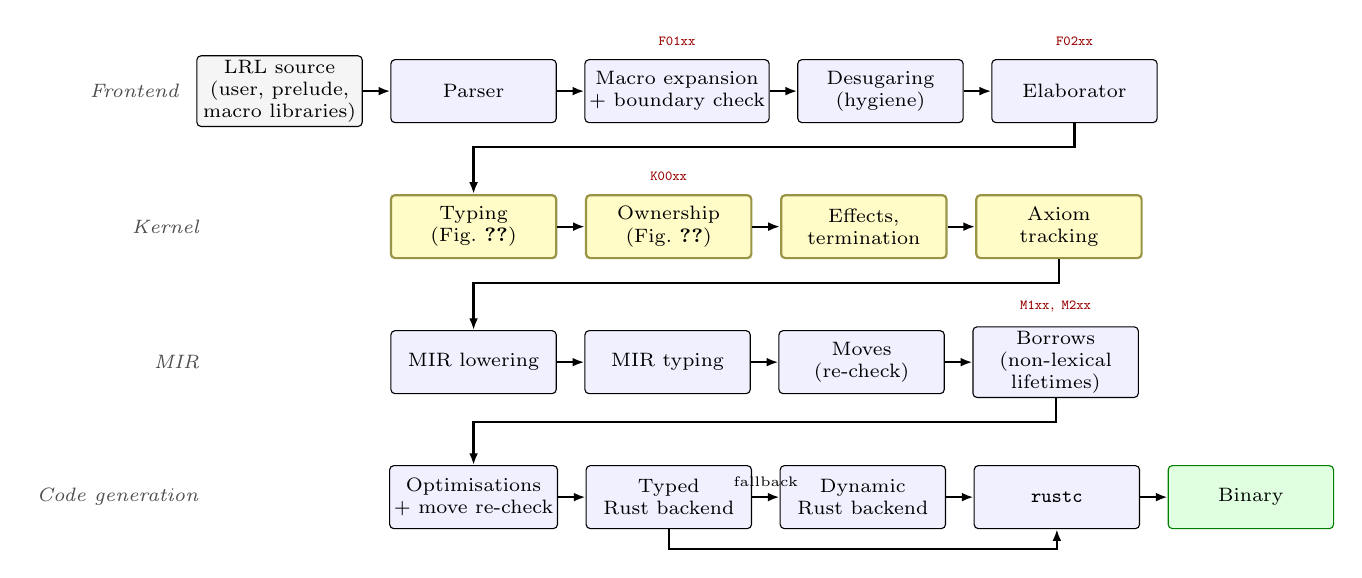
\begin{tikzpicture}[
  font=\scriptsize,
  >={Latex[length=1.5mm]},
  node distance=5mm and 3.5mm,
  box/.style={draw, rounded corners=1.5pt, minimum height=8mm, minimum width=21mm,
              align=center, inner sep=1.5pt, fill=white},
  input/.style={box, fill=gray!8},
  untrusted/.style={box, fill=blue!6},
  trusted/.style={box, fill=yellow!22, draw=yellow!55!black, thick},
  output/.style={box, fill=green!12, draw=green!50!black},
  flow/.style={->, thick},
  band/.style={font=\scriptsize\itshape, anchor=east, text=black!70},
  err/.style={font=\tiny, text=red!60!black},
]
% row 1: frontend
\node[input]                  (src)   {LRL source\\(user, prelude,\\macro libraries)};
\node[untrusted, right=of src] (parse) {Parser};
\node[untrusted, right=of parse] (mac) {Macro expansion\\+ boundary check};
\node[untrusted, right=of mac] (des)  {Desugaring\\(hygiene)};
\node[untrusted, right=of des] (elab) {Elaborator};
% row 2: kernel
\node[trusted, below=9mm of parse] (ktype) {Typing\\(Fig.~\ref{fig:typing})};
\node[trusted, right=of ktype] (kown) {Ownership\\(Fig.~\ref{fig:own})};
\node[trusted, right=of kown] (keff) {Effects,\\termination};
\node[trusted, right=of keff] (kax) {Axiom\\tracking};
% row 3: MIR
\node[untrusted, below=9mm of ktype] (low) {MIR lowering};
\node[untrusted, right=of low] (mty) {MIR typing};
\node[untrusted, right=of mty] (mmv) {Moves\\(re-check)};
\node[untrusted, right=of mmv] (mbr) {Borrows\\(non-lexical\\lifetimes)};
% row 4: codegen
\node[untrusted, below=9mm of low] (opt) {Optimisations\\+ move re-check};
\node[untrusted, right=of opt] (typed) {Typed\\Rust backend};
\node[untrusted, right=of typed] (dyn) {Dynamic\\Rust backend};
\node[untrusted, right=of dyn] (rustc) {\texttt{rustc}};
\node[output, right=of rustc] (bin) {Binary};
% flows
\draw[flow] (src) -- (parse);
\draw[flow] (parse) -- (mac);
\draw[flow] (mac) -- (des);
\draw[flow] (des) -- (elab);
\draw[flow] (elab.south) -- ++(0,-3mm) -| (ktype.north);
\draw[flow] (ktype) -- (kown);
\draw[flow] (kown) -- (keff);
\draw[flow] (keff) -- (kax);
\draw[flow] (kax.south) -- ++(0,-3mm) -| (low.north);
\draw[flow] (low) -- (mty);
\draw[flow] (mty) -- (mmv);
\draw[flow] (mmv) -- (mbr);
\draw[flow] (mbr.south) -- ++(0,-3mm) -| (opt.north);
\draw[flow] (opt) -- (typed);
\draw[flow] (typed) -- (dyn) node[midway, above, font=\tiny] {fallback};
\draw[flow] (dyn) -- (rustc);
\draw[flow] (typed.south) -- ++(0,-2.5mm) -| (rustc.south);
\draw[flow] (rustc) -- (bin);
% error codes
\node[err, above=0.5mm of mac] {\texttt{F01xx}};
\node[err, above=0.5mm of elab] {\texttt{F02xx}};
\node[err, above=0.5mm of kown] {\texttt{K00xx}};
\node[err, above=0.5mm of mbr] {\texttt{M1xx}, \texttt{M2xx}};
% bands
\node[band, left=1mm of src.west] {Frontend};
\node[band] at ($(ktype.west)+(-23mm,0)$) {Kernel};
\node[band] at ($(low.west)+(-23mm,0)$) {MIR};
\node[band] at ($(opt.west)+(-23mm,0)$) {Code generation};
\end{tikzpicture}
\caption{The LRL pipeline. The kernel (yellow) is the logical trusted base (\S\ref{sec:own:trust}). Every definition and top-level expression passes through all stages up to the borrow check; code is generated only for definitions that pass every check (Proposition~\ref{prop:pipeline}). The labels show where the main families of diagnostic codes are reported; MIR lowering reports the program shapes it does not support without a code. With \texttt{-{}-backend auto}, the dynamic backend is used when the typed backend or \texttt{rustc} rejects a program.}
\label{fig:pipeline}
\end{figure*}

\paragraph{Elaboration.}
The elaborator turns surface syntax into kernel terms.
It is bidirectional---it has separate inference and checking modes, with metavariables for unknown types and implicit arguments and with postponed unification constraints---and it inserts implicit arguments, infers the kinds of unannotated $\lambda$s with the analysis of Definition~\ref{def:req}, inserts kind coercions (\S\ref{sec:core:kinds}), and translates \lstinline|match| into recursor applications.
A \lstinline|match| with an explicit motive, \lstinline|(match e (motive M) ...)|, becomes a recursor application with motive \lstinline|M|, so that each case is checked against the motive at its constructor; without \lstinline|motive|, the return type is constant.
The elaborator is outside the logical trusted base: its output is checked by the kernel.

\paragraph{Kernel.}
The kernel checks a definition in the order shown in Figure~\ref{fig:pipeline}: the type of the definition, its value (Figure~\ref{fig:typing}), its ownership (Figure~\ref{fig:own}), the well-formedness of the capture annotations recorded by the elaborator, effects (total code may not call partial or unsafe code), and termination of total definitions; it also records axiom dependencies.
Inductive declarations are checked for positivity and universe consistency, and their recursors and Copy instances are derived.
The kernel source has the size shown in Table~\ref{tab:scale}; without the unit tests and test helpers inside the crate it has \NumKernelNonTestLines{} lines.
The kernel is the part of the compiler that must be read to trust its guarantees; at this size, that is a substantial but feasible effort, and we do not claim that it is minimal.

\paragraph{MIR.}
Lowering produces one MIR body per definition and one per closure.
Inductive values become tagged unions whose runtime type ignores indices; proofs become unit values.
Recursor applications are compiled as described in \S\ref{sec:own:rec}: for a non-recursive type, a switch with one inline branch per constructor; for a recursive type, a call to a generated recursive function that takes the minor premises as closures and computes induction hypotheses before calling them.
After the mandatory analyses (\S\ref{sec:own:borrow}), MIR is optimised by erasure of proof locals, dead-code elimination, control-flow simplification and a conservative copy propagation; the ownership analysis is then run again.

\paragraph{Two backends.}
Both backends generate Rust source from the same checked MIR and call \texttt{rustc}.
The \emph{typed} backend maps inductive types to Rust enumerations (recursive fields behind reference-counted pointers, \lstinline|Rc|), \lstinline|Nat| to a 64-bit unsigned integer, and functions to reference-counted closure objects.
The \emph{dynamic} backend maps every value to one universal Rust enumeration.
The dynamic backend exists because the typed one does not cover every MIR shape; with \texttt{-{}-backend auto} the compiler tries the typed backend first and falls back to the dynamic one, with a warning, if typed code generation or \texttt{rustc} fails.
A conformance test runs a set of programs through both backends and compares their results.
Neither backend is part of the logical trusted base, and the dynamic fallback does not weaken any check: both backends start from MIR that has passed all the analyses.

\paragraph{Using LRL.}
We write \texttt{lrl} for the compiler's command-line program, which \texttt{cargo build -p cli} builds under the name \texttt{cli}.
\texttt{lrl compile} produces a native binary whose entry point is the last top-level definition; \texttt{lrl run -{}-backend typed} (or \texttt{auto}) compiles the file and runs the binary.
\texttt{lrl run} with its default setting, \texttt{-{}-backend dynamic}, does not generate code: after all checks it normalises the file's top-level expressions with the kernel's evaluator and prints the results, without executing the entry definition.
Without a file, \texttt{lrl} starts a read--eval--print loop, which accepts definitions and expressions one at a time and can show the type of an expression or its expansion.
The flags \texttt{-{}-expand-1} and \texttt{-{}-expand-full} print the result of one step or of the whole of macro expansion, and \texttt{-{}-trace-macros} prints every expansion step; these are the main tools for debugging macros.
Most diagnostics carry a code whose prefix names the component that reports them: \texttt{F} for the frontend, \texttt{K} for the kernel, \texttt{M} for the MIR analyses, and \texttt{C} for the driver's own checks, such as those of macro imports and of \texttt{-{}-panic-free}. A few errors are printed without a code, among them the errors of MIR lowering, which rejects some program shapes that it does not support (\S\ref{sec:own:borrow}). Where it is known, a diagnostic also gives the source location and, for code produced by a macro, the macro's name and call site.
All commands exit with a non-zero status if any check fails.
